\documentclass[12pt]{article}

\usepackage{times}
\usepackage{graphicx}
\usepackage{amsmath}
\usepackage{url}

\setlength{\textwidth}{6.5in}
\setlength{\textheight}{8.9in}
\setlength{\oddsidemargin}{0.0in}
\setlength{\topmargin}{0.05in}
\setlength{\headheight}{-0.05in}
\setlength{\headsep}{0.0in}

\newcommand{\indep}{\perp\!\!\!\perp}

\begin{document}

\begin{center}
{\bf CS 6300} \hfill {\large\bf HW09: VPI and HMMs \hfill Due April 20, 2021}
\end{center}

\noindent
Please use the \LaTeX\ template to produce your writeups. See the
Homework Assignments page on the class website for details.  Hand in
via gradescope.

\section{Decision Networks and VPI}

\begin{center}
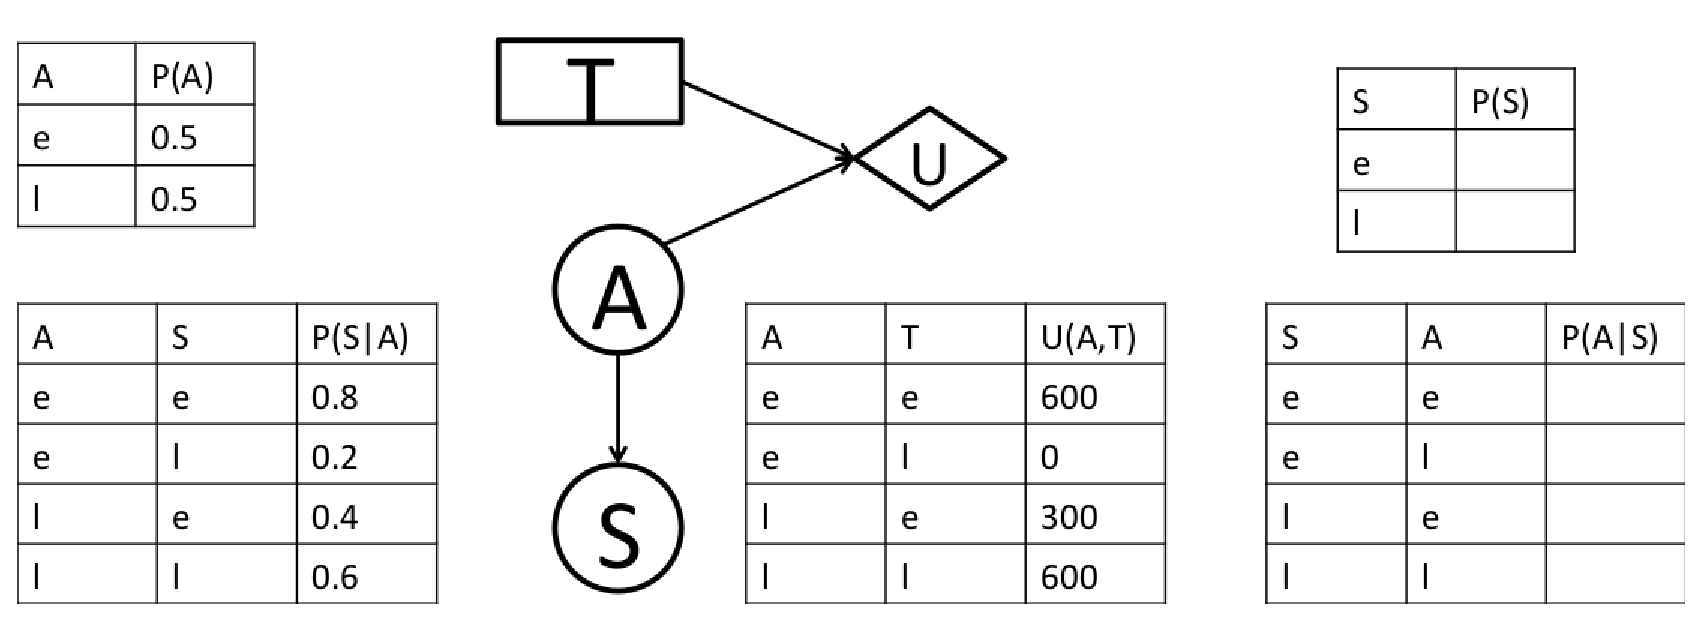
\includegraphics[width=6in]{influence-diagram-w-additional-tables.eps}
\end{center}

Your parents are visiting you for graduation.  You are in charge of
picking them up at the airport.  Their arrival time ($A$) might be
early ($e$) or late ($l$).  You decide on a time ($T$) to go to the
airport, also either early ($e$) or late ($l$).  Your sister ($S$) is
a noisy source of information about their arrival time. The
probability values and utilities are shown in the tables above.

\begin{enumerate}

\item Fill in the above empty table entries by computing $P(S), P(A|S)$ and then compute the quantities below. 

\begin{tabular}{|r|r|} \hline
S  & $P(S)$ \\ \hline
e &   $0.8 * 0.5 + 0.4 * 0.5 = 0.6$    \\ \hline
l &   $0.2 * 0.5 + 0.6 * 0.5 = 0.4$   \\ \hline
\end{tabular}

\begin{tabular}{|r|r|r|} \hline
S & A & $P(A|S)$ \\ \hline
e & e & $(0.8 * 0.5) / 0.6 = 0.667$ \\ \hline
e & l & $(0.4 * 0.5) / 0.6 = 0.333$ \\ \hline
l & e & $(0.2 * 0.5) / 0.4 = 0.25$ \\ \hline
l & l & $(0.6 * 0.5) / 0.4 = 0.75$ \\ \hline
\end{tabular}

\begin{enumerate}

\item $EU(T=e) = \Sigma_a P(a) * EU(a, T = e) = 0.5 * 600 + 0.5 * 300 = 450$

\item $EU(T=l) = \Sigma_a P(a) * EU(a, T = l) = 0.5 * 0 + 0.5 * 600 = 300$

\item $MEU( \{ \} ) = max(EU) = 450$

\item Optimal action with no observations: \textbf{Go early.}

\end{enumerate}

\item Now we consider the case where you decide to ask your sister for input.

\begin{enumerate}

\item $EU(T=e | S = e) = \Sigma_a P(a) * EU(a, T = e, s = e) = 0.667 * 600 + 0.333 * 300 = 500$

\item $EU(T=l | S = e) = \Sigma_a P(a) * EU(a, T = l, S = e) = 0.667 * 0 + 0.333 * 600 = 200$

\item $MEU( \{ S=e \} ) = max(EU | S=e) = 500$

\item Optimal action with observation $\{S = e\}$: \textbf{Go early}

\item $EU(T = e | S = l =  \Sigma_a P(a) * EU(a, T = e, s = e) = 0.25 * 600 + 0.75 * 300 = 375$

\item $EU(T = l | S = l) =  \Sigma_a P(a) * EU(a, T = l, S = e) = 0.25 * 0 + 0.75 * 600 = 450$

\item $MEU( \{ S=l \} ) = max(EU | S=l) = 450$

\item Optimal action with observation $S = l$: \textbf{Go late}

\item $VPI(S) = (0.6 * 500) + (0.4 * 450) - 450 = 30$

\end{enumerate}

\end{enumerate}

% \clearpage

% \section{HMMs}

% Romeo and Juliet are two lovesick robots; they function best when each
% knows where the other is.  Romeo has become lost, and is trying to
% figure out where he is so he can tell Juliet.  Romeo is on the grid
% below, which also lists transition probabilities and properties of the
% sensors.  At each step, Romeo senses, and then transitions to an
% adjacent room to get to the next time step.  Romeo observed the
% following evidence while wandering in grief over his inability to tell
% Juliet where he is: 2 walls, 2 walls, 3 walls.

% \begin{enumerate}

% \item Forward Algorithm: Compute the most likely location, given the evidence.

% \item Viterbi Algorithm: Compute the most likely sequence of steps he
%   took in the maze for the above evidence.

% \end{enumerate}

% \begin{center}
% \includegraphics[height=7in]{Romeo.eps}
% \end{center}

\end{document}


